\section{\ce{[Zn(N_3)_2(4-methoxypyridine)_2]}}
\subsection{Synthesis}
\ce{Zn(NO_3)_2*6 H_2O} (0.59 g, 2 mmol), \ce{NaN_3} (0.13 g, 2 mmol) and  4-methoxy-pyridine (0.22 g, 2 mmol) were added in 40 mL distilled \ce{H_2O}. The solution was heated up to 80$^\circ$C  and stirred for 2 hours. After filtration the clear solution was stirred again for 30 minutes at the same temperature and then cooled down to RT. After 3 days needle-shaped white crystals were obtained. Anal. Calculated for \ce{C_{12}H_{14}N_8O_2Zn} (367.70 g/mol) : 39.20\% C; 3.84\% H; 30.48\% N; Found: 38.96\% C; 3.87\% H; 30.33 \% N; IR (ATR, cm$^{-1}$): 2094 (s), 2058 (s), 1615 (s), 1568 (s), 1513 (s), 1439 (s), 1355 (m), 1298 (s), 1210 (s), 1061 (m), 1031 (s), 819 (s), 731 (w), 659 (w), 580 (w), 535 (s), 465 (m)

\begin{figure}[h!]
\centering
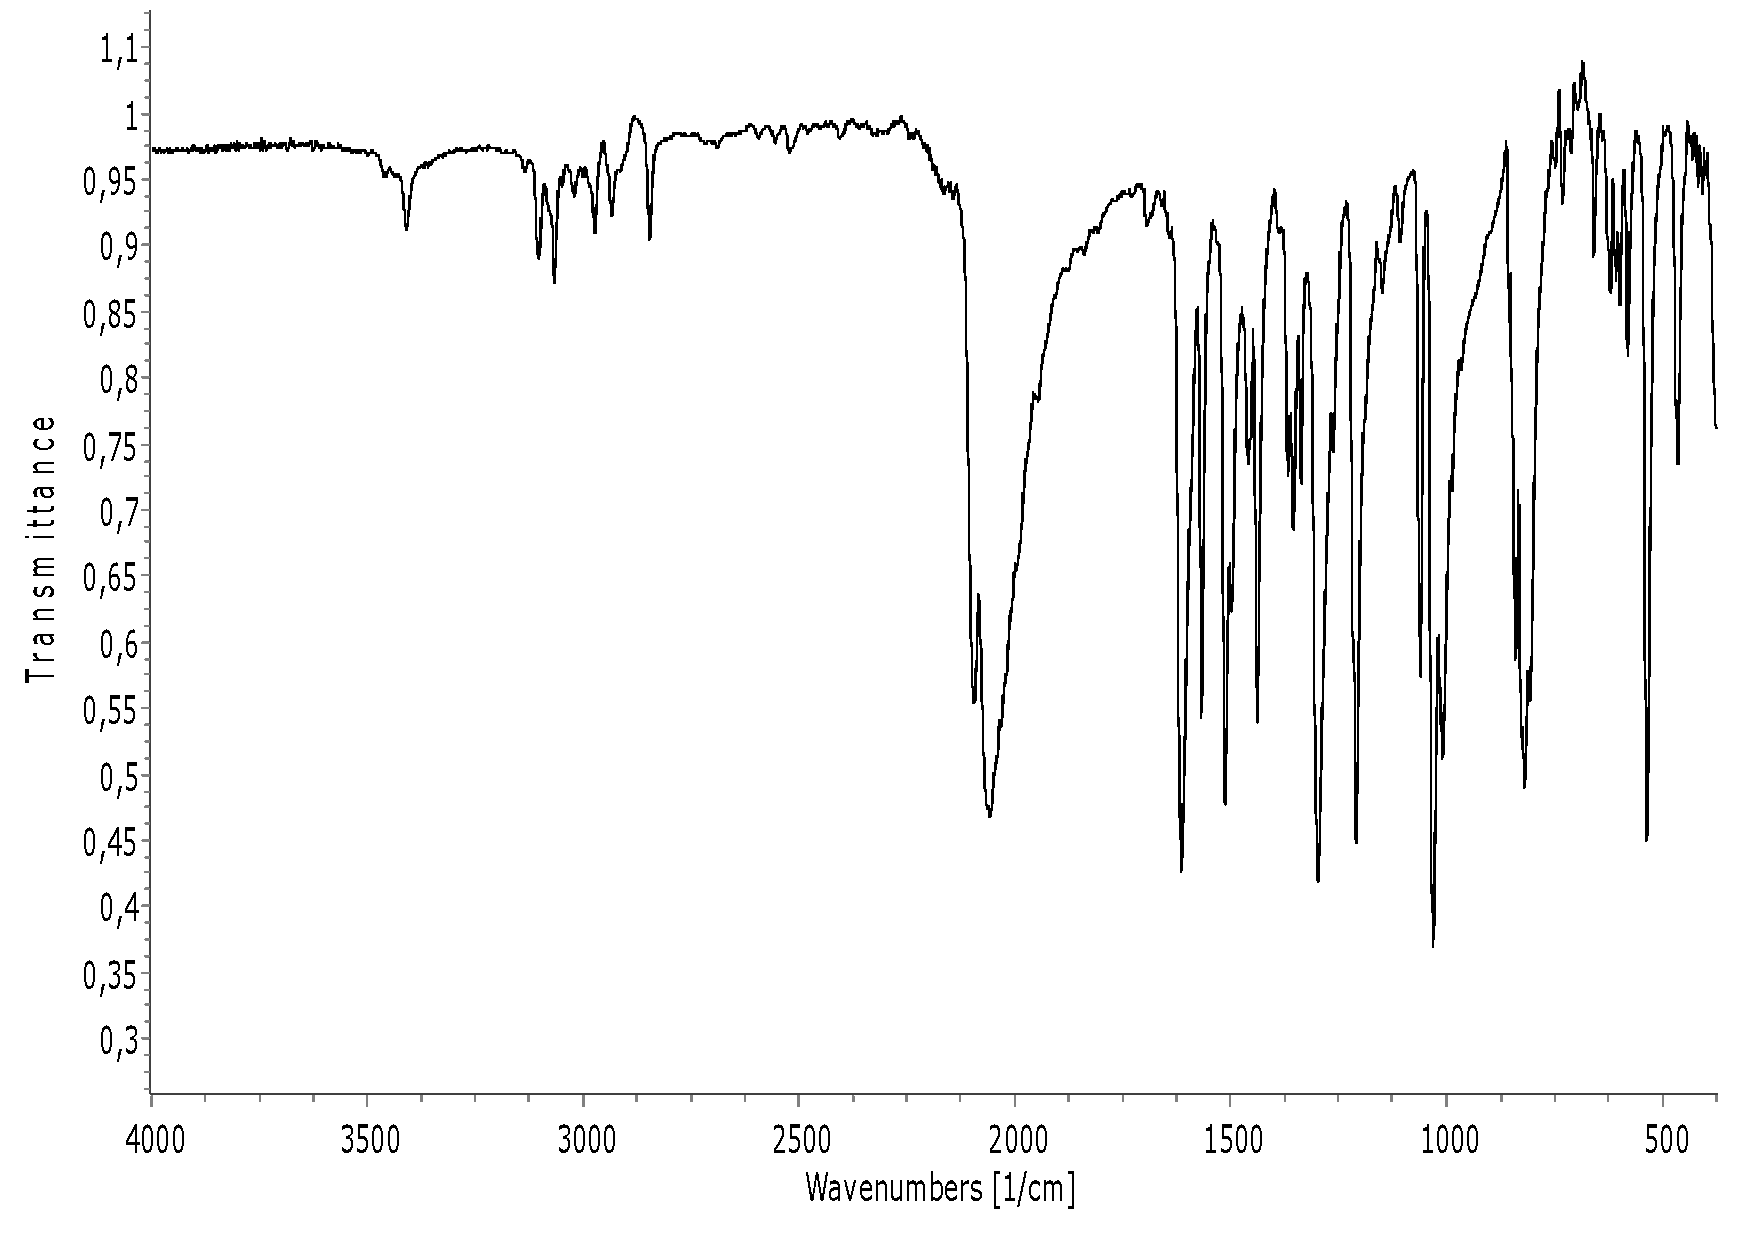
\includegraphics[width=1\textwidth]{figures/ZnA4MOP-IR.pdf}
\caption{IR spectrum of \ce{[Zn(N_3)_2(4-MeOpy)_2]}}
\end{figure}

\subsection{Structural characterization}

The crystal structure of \ce{[Zn(N_3)_2(4-MeOpy)_2]} consists of mononuclear and neutral Zn(II) complexes, as depicted in figure \ref{fig:ZnA4MOP_pv} (perspective view) and figure \ref{fig:ZnA4MOP_packv} (packing view). Selected bond parameters are listed in table \ref{batab:ZnA4MOP}.  Zn(1) is tetrahedrally coordinated by N(11) and N(21) of two terminal azido groups, further by N(1) and N(2) atoms of two neutral \ce{4-methoxypyridine} molecules. The Zn-N bond lengths range from 1.9330(14) to 2.0311(13) \AA, and the bond angles within the \ce{ZnN_4} tetrahedron vary from 100.25(6) to 128.66(6)$^\circ$. The bond parameters of the terminal azido groups are: Zn-N-N = 138.48(12) and 142.44(12)$^\circ$, N-N-N = 177.17(17) and 174.52(17)$^\circ$, N(x1)-N(x2) = 1.182(2) and 1.1918(19) \AA, N(x2)-N(x3) = 1.156(2) and 1.148(2) \AA.The shortest metal-metal separation is 5.3288(7) \AA. 

\begin{table}[htpb!]
\centering
\captionabove{Selected bond lengths (\AA) and angles ($^\circ$) for \ce{[Zn(N_3)_2(4-MeOpy)_2]}}
\begin{tabular}{|l|l|l|l|}
\hline
Zn(1)-N(11) & 1.9714(14) & Zn(1)-N(1) & 2.0311(13)\\
\hline
Zn(1)-N(21) & 1.9330(14) & Zn(1)-N(2) & 2.0192(13)\\
\hline
N(11)-N(12) & 1.182(2) & N(12)-N(13) & 1.156(2)\\
\hline
N(21)-N(22) & 1.1918(19) & N(22)-N(23) & 1.148(2)\\
\hline
\hline
N(11)-Zn(1)-N(21) & 128.66(6) & N(1)-Zn(1)-N(21) & 101.00(5)\\
\hline
N(2)-Zn(1)-N(21) & 110.32(6) & N(1)-Zn(1)-N(11) & 100.25(6)\\
\hline
N(2)-Zn(1)-N(11) & 104.01(6) & N(1)-Zn(1)-N(2) & 111.79(5)\\
\hline
Zn(1)-N(11)-N(12) & 138.48(12) & N(11)-N(12)-N(13) & 177.17(17)\\
\hline
Zn(1)-N(21)-N(22) & 142.44(12) & N(21)-N(22)-N(23) & 174.52(17)\\
\hline
\end{tabular}

\label{batab:ZnA4MOP}
\end{table}



\begin{figure}[!htpb]
\centering
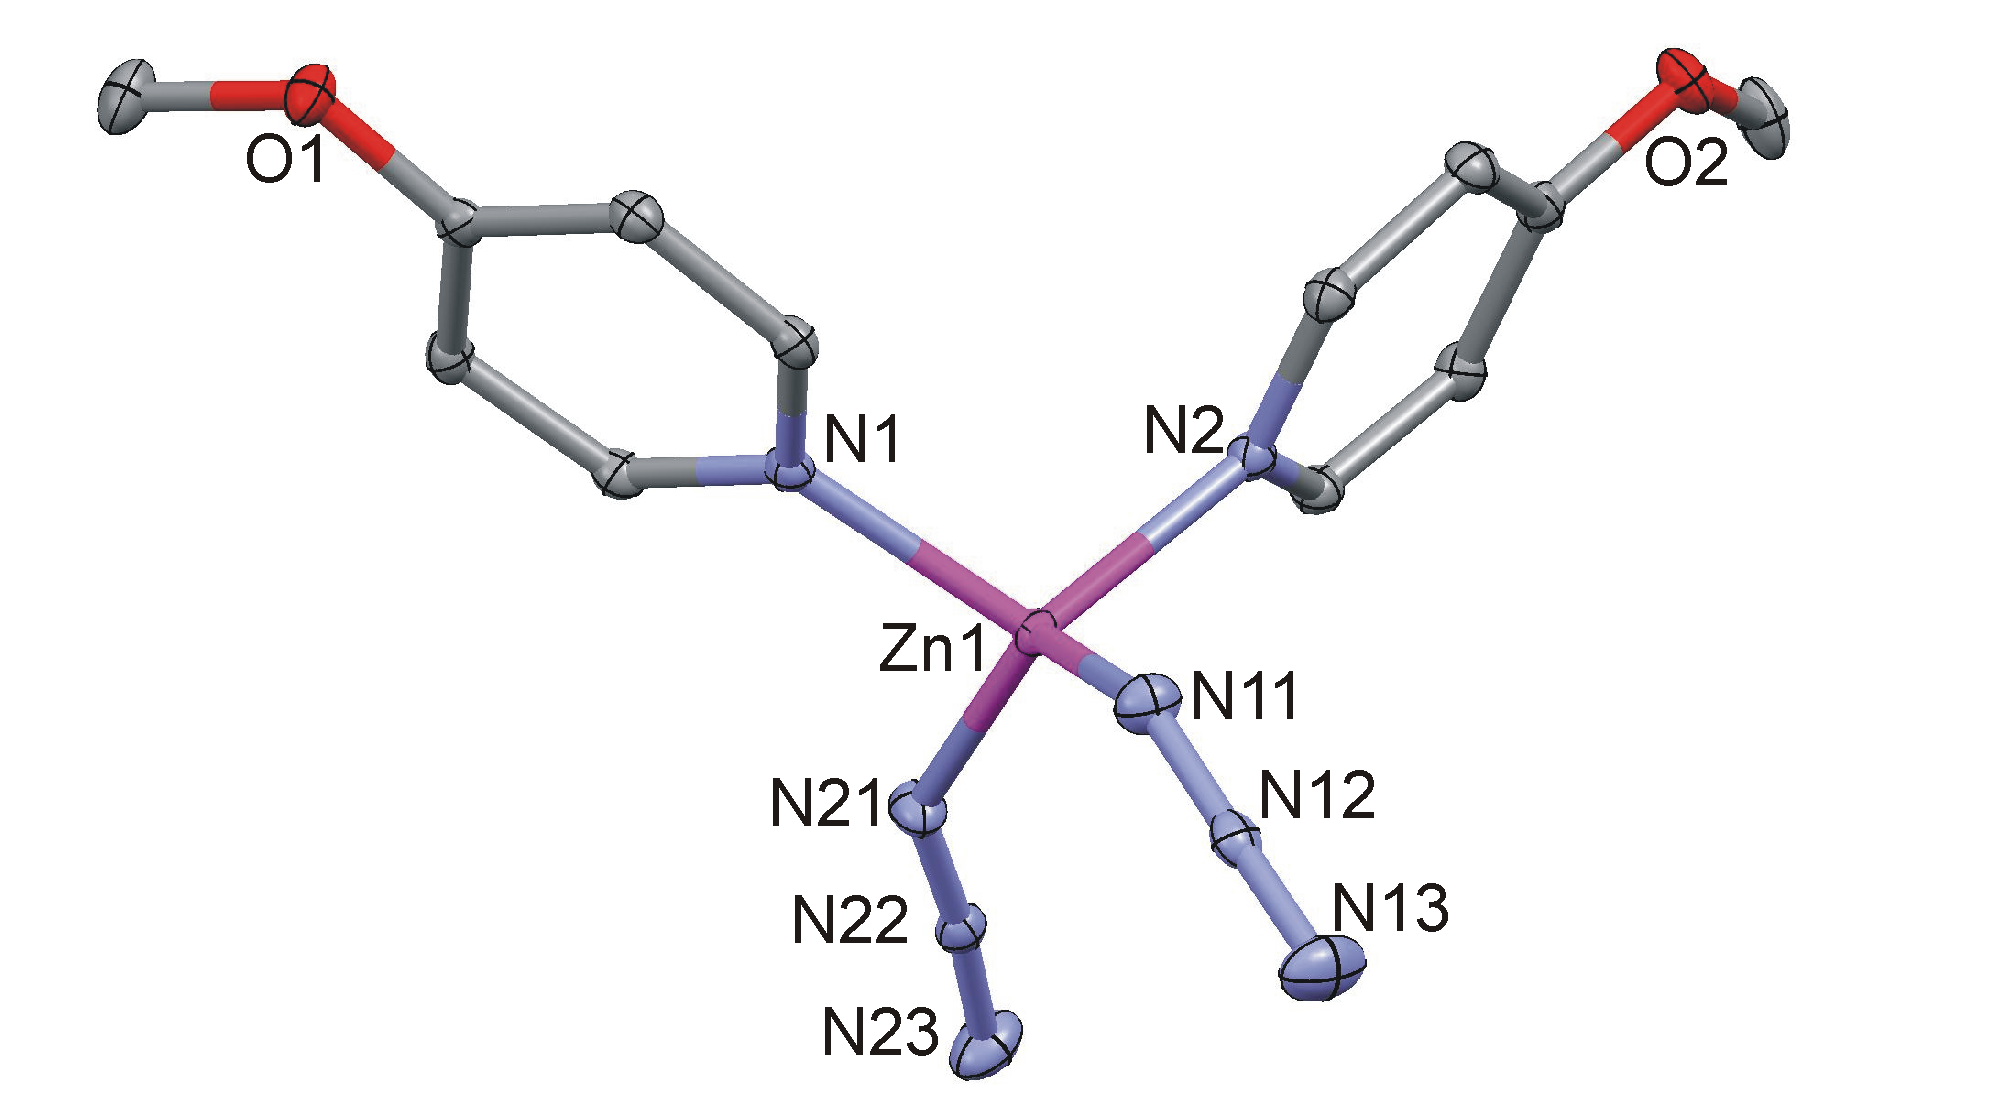
\includegraphics[width=1\textwidth]{figures/Zn_4OMP_FIGm11.png}
\caption[Perspective view of \ce{[Zn(N_3)_2(4-MeOpy)_2]}]{Perspective view of \ce{[Zn(N_3)_2(4-MeOpy)_2]} with the atom numbering scheme. Symmetry codes: (‘): -x,y,-z+1/2; (“): 1-x,y,-z+1/2.}
\label{fig:ZnA4MOP_pv}
\vspace{\floatsep}
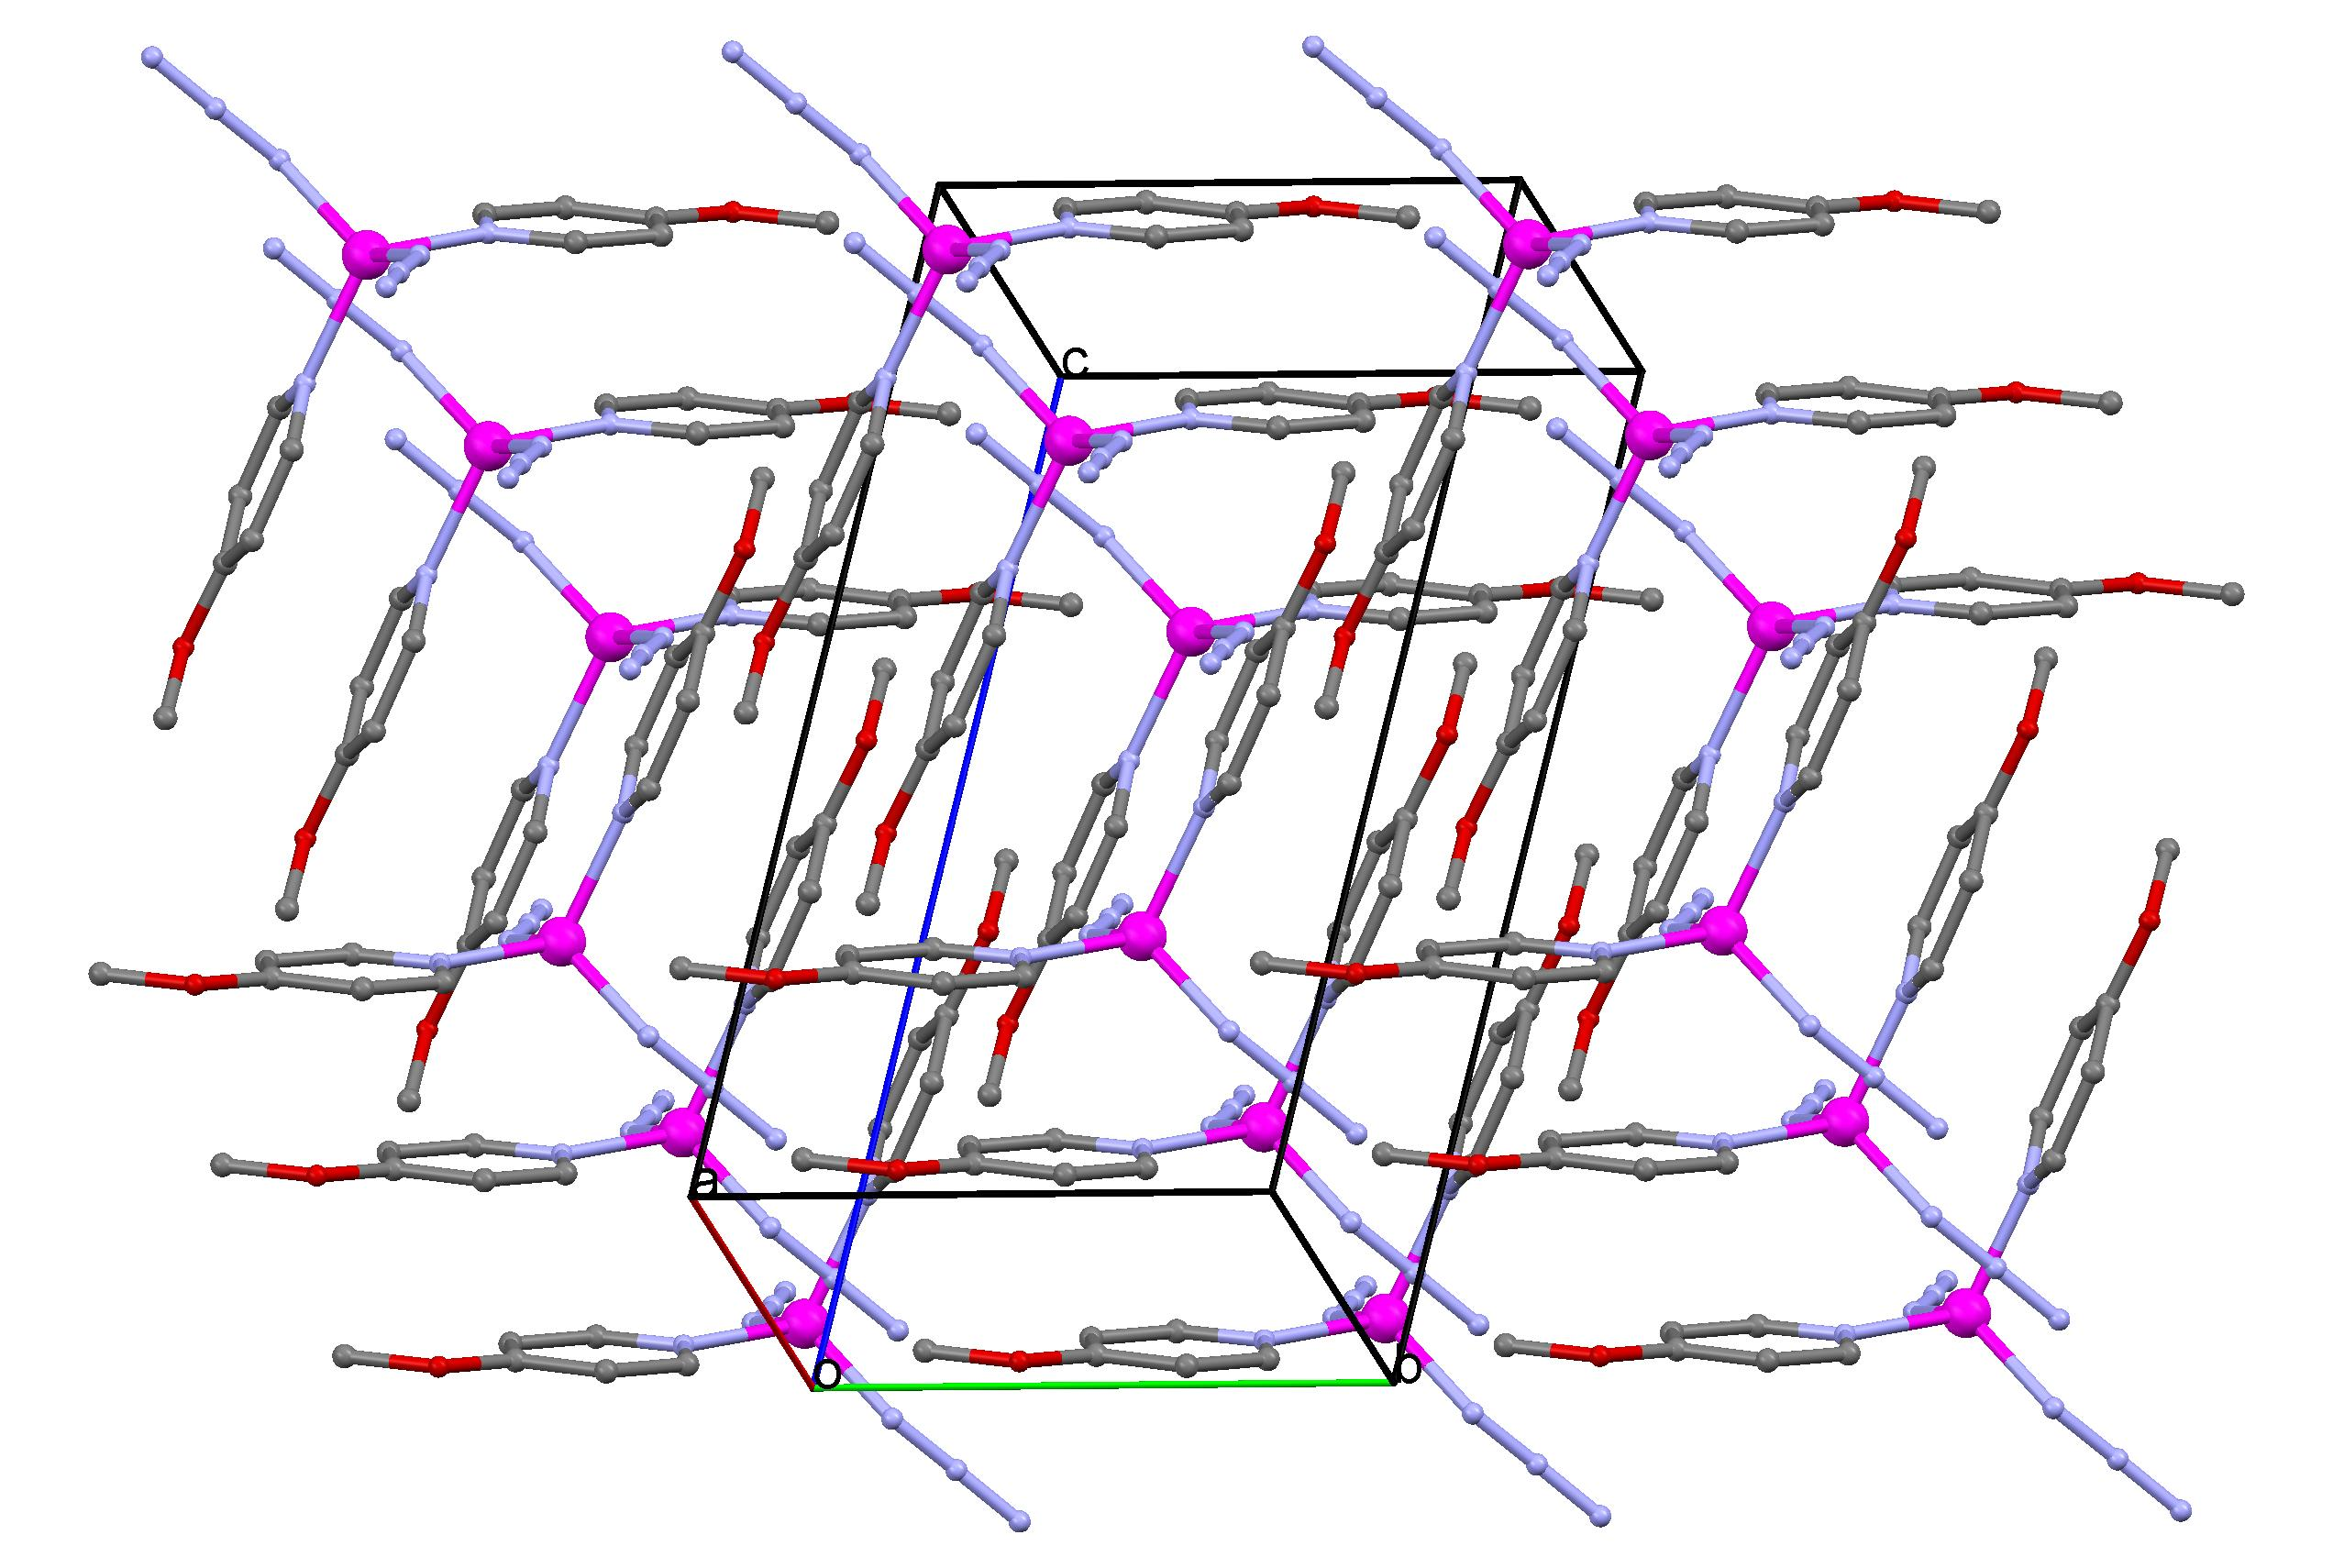
\includegraphics[width=1\textwidth]{figures/zn_A4meop_CA.png}
\caption{Packing view of \ce{[Zn(N_3)_2(4-MeOpy)_2]}.}
\label{fig:ZnA4MOP_packv}
\end{figure}

\renewcommand{\arraystretch}{1.5}
\begin{table}
\centering
\captionabove{Crystallographic data and processing parameter of \ce{[Zn(N_3)_2(4-MeOpy)_2]}}
\begin{tabular}{ | l |  l | }
\hline
Empirical formula & \ce{C_{12}H_{14}N_{8}O_{2}Zn}\\
\hline
Formula mass & 367.70\\
\hline
System & triclinic\\
\hline
Space group & P-1\\
\hline
a ({\AA}) & 5.3288(7)\\
\hline
b ({\AA}) & 9.751(1)\\
\hline
c ({\AA}) & 15.1580(14)\\
\hline
$\alpha$ ($^\circ$) & 88.877(3)\\
\hline
$\beta$ ($^\circ$) & 82.068(3)\\
\hline
$\gamma$ ($^\circ$) & 78.448(3)\\
\hline
V (\AA$^{3}) $  & 764.26(15)\\
\hline
Z & 2\\
\hline
T (K) & 100(2)\\
\hline
$\mu$ (mm$^{-1}$) & 1.630\\
\hline
 D$_{calc}$ (Mg/m$^{3}$) & 1.598\\
\hline
Crystal size (mm) & 0.32 x 0.22 x 0.18\\
\hline
$\theta$ max ($^\circ$) & 26.35\\
\hline
Data collected & 6131\\
\hline
Unique refl./ R$_{int}$ & 3069 / 0.0172\\
\hline
Parameters & 210\\
\hline
Goodness-of-Fit on F$^{2}$ & 1.063\\
\hline
R1 / wR2 (all data) & 0.0220 /0.0542\\
\hline
Residual extrema (e/\AA$^{3}$) & 0.27 /-0.40\\
\hline
\end{tabular}

\label{ptab:ZnA4MOP}


\end{table}


